% Software Overview
% MIT License
%
% Copyright (c) 2026 HumberASV
% Copyright (c) 2026 Carson Fujita
%
% Permission is hereby granted, free of charge, to any person obtaining a copy
% of this software and associated documentation files (the "Software"), to deal
% in the Software without restriction, including without limitation the rights
% to use, copy, modify, merge, publish, distribute, sublicense, and/or sell
% copies of the Software, and to permit persons to whom the Software is
% furnished to do so, subject to the following conditions:
%
% The above copyright notice and this permission notice shall be included in all
% copies or substantial portions of the Software.
%
% THE SOFTWARE IS PROVIDED "AS IS", WITHOUT WARRANTY OF ANY KIND, EXPRESS OR
% IMPLIED, INCLUDING BUT NOT LIMITED TO THE WARRANTIES OF MERCHANTABILITY,
% FITNESS FOR A PARTICULAR PURPOSE AND NONINFRINGEMENT. IN NO EVENT SHALL THE
% AUTHORS OR COPYRIGHT HOLDERS BE LIABLE FOR ANY CLAIM, DAMAGES OR OTHER
% LIABILITY, WHETHER IN AN ACTION OF CONTRACT, TORT OR OTHERWISE, ARISING FROM,
% OUT OF OR IN CONNECTION WITH THE SOFTWARE OR THE USE OR OTHER DEALINGS IN THE
% SOFTWARE.

% setup section for software development
\subsection{Docker Use}
\label{sec:docker-setup}

Docker is a powerful tool for creating, deploying, and running applications in containers. It allows you to package your application with all of its dependencies into a standardized unit for software development \autocite{ABOUTDOCKER}.
This can be particularly useful for ROS 2 development, as it can help ensure that your development environment is consistent across different machines and operating systems.

\warningbox{It is prerequisite to have an understanding of Linux systems before using Docker.}

\notebox{This document explains the underlying configuration required for the project. For most developers, the \texttt{LoonEnv} tool (Section \ref{sec:loon-env}) automates this setup, including Docker installation and network optimization.}

\bigskip
\subsubsection{Images}

Docker images are the basis of Docker containers. They are read-only templates that contain the instructions for creating a Docker container. You can create your own Docker images or use pre-built images from Docker Hub. For ROS 2 development, you can use the official ROS 2 images provided by Open Robotics or, for NVIDIA Jetson devices, images provided by NVIDIA. These images come pre-configured with ROS 2 and the necessary dependencies, making it easier to get started with development.

We have used our own custom image based on the official ROS 2 image, which includes additional tools and libraries that we find useful for our development process. You can find our custom Dockerfile when we release our \href{https://github.com/HumberASV/Loon-Env}{Loon-Env} repository.

\notebox{For our NVIDIA Orin Nano, we are using \url{nvcr.io/nvidia/isaac/ros:aarch64-ros2_humble_4c0c55dddd2bbcc3e8d5f9753bee634c}, which is based on the official ROS-2 Humble image and includes additional tools and libraries for Loon-E's development on NVIDIA Jetson devices.}

\subsubsection{Volumes}

Docker volumes are a way to persist data generated by and used by Docker containers. They allow you to store data outside of the container's filesystem, which can be useful for sharing data between the host machine and the container or for persisting data across container restarts. When using Docker for ROS 2 development, you can use volumes to share your ROS 2 workspace between the host machine and the container. This allows you to edit your code on the host machine and have those changes reflected in the container without needing to rebuild the image.

Because Loon-E uses Zedx we have to make volumes to ensure the Zedx SDK and its dependencies are properly shared between the host machine and the container. This is necessary because the Zedx SDK requires access to certain hardware resources, such as the GPU, which may not be available within the container. By using volumes, we can ensure that the necessary files and libraries are accessible to the container, allowing us to use the Zedx SDK for vision processing in our ROS 2 development.

Following the example on \href{https://www.stereolabs.com/docs/cameras/zed-x/zed-x-and-docker}{Stereolabs}, we need to set the following volumes.

\begin{landscape}

\subsubsection{Hardware \& Device Volumes}

\begin{table}[H]
    \centering
    \begin{tabular}{|l|l|p{9cm}|}
        \hline
        \textbf{Volume Name} & \textbf{Mount Path} & \textbf{Purpose} \\
        \hline
        /dev/ & /dev/ & This is the device file for the Zedx camera. It allows the container to access the camera hardware. \\
        \hline
        /tmp/ & /tmp/ & Temporary directory that the Zedx SDK uses for storing temporary files. It allows the container to access these files as needed. \\
        \hline
    \end{tabular}
    \caption{Docker Hardware Volumes for Zedx SDK}
    \label{tab:docker-volumes-hardware}
\end{table}

\subsubsection{SDK Configuration Volumes}

\begin{table}[H]
    \centering
    \begin{tabular}{|l|l|p{9cm}|}
        \hline
        \textbf{Volume Name} & \textbf{Mount Path} & \textbf{Purpose} \\
        \hline
        /var/nvidia/nvcam/settings/ & /var/nvidia/nvcam/settings/ & Directory where the Zedx SDK stores its configuration files. It allows the container to access these files as needed. \\
        \hline
        /etc/systemd/system/zed\_x\_daemon.service & /etc/systemd/system/zed\_x\_daemon.service & Systemd service file for the Zedx daemon. It allows the container to manage the Zedx daemon as needed. \\
        \hline
        \${HOME}/zed\_docker\_ai/ & /usr/local/zed\_docker\_ai/ & Host directory used for storing any additional files or data related to ROS 2 development with the Zedx SDK. It allows easy sharing between host and container. \\
        \hline
    \end{tabular}
    \caption{Docker SDK Configuration Volumes for Zedx SDK}
    \label{tab:docker-volumes-config}
\end{table}

\subsubsection{Display \& X11 Volumes}

\begin{table}[H]
    \centering
    \begin{tabular}{|l|l|p{9cm}|}
        \hline
        \textbf{Volume Name} & \textbf{Mount Path} & \textbf{Purpose} \\
        \hline
        \${HOME}/.Xauthority & /root/.Xauthority & X authority file for the host machine. It allows the container to access the X server for running graphical applications. \\
        \hline
    \end{tabular}
    \caption{Docker Display Volumes for Zedx SDK}
    \label{tab:docker-volumes-display}
\end{table}

\end{landscape}

\subsubsection{Options}

When running a Docker container for ROS 2 development, there are several options that you may need to set to ensure that the container has the necessary permissions and access to resources. These options can include runtime settings, network settings, and GPU access.

\begin{table}[H]
    \centering
    \begin{tabular}{|l|p{10cm}|}
        \hline
        \textbf{Option Name} & \textbf{Purpose} \\
        \hline
        --runtime nvidia & Allows the container to use the NVIDIA runtime, necessary for accessing GPU resources required by the Zedx SDK. \\
        \hline
        -it & Interactive terminal for running commands and debugging within the container. \\
        \hline
        --privileged & Gives the container additional privileges, which may be necessary for accessing hardware resources or managing system services. \\
        \hline
        --net=host & Uses the host machine's network stack, useful for communication between the container and other devices on the network. \\
        \hline
        --ipc=host & Uses the host machine's IPC namespace, necessary for applications that require shared memory or other IPC mechanisms. \\
        \hline
        --gpus all & Allows the container to access all available GPU resources on the host machine. \\
        \hline
        --pid=host & Uses the host machine's PID namespace, useful for applications that require access to the host's process information or for debugging. \\
        \hline
    \end{tabular}
    \caption{Docker Options for ROS 2 Development}
    \label{tab:docker-options}
\end{table}

\subsubsection{Environment Variables}
\label{sec:docker-env-vars}
When running a Docker container for ROS 2 development, you may need to set certain environment variables to ensure that the container has the necessary configuration and access to resources. 

\begin{table}[H]
    \centering
    \begin{tabular}{|l|p{10cm}|}
        \hline
        \textbf{Environment Variable} & \textbf{Purpose} \\
        \hline
        DISPLAY & Allows the container to access the host machine's display, useful for running graphical applications or visualizing data from the Zedx camera. \\
        \hline
        XAUTHORITY & Allows the container to access the host machine's X authority file, necessary for running graphical applications that require access to the X server. \\
        \hline
        \texttt{ROS\_DOMAIN\_ID} & Sets the ROS domain ID for the container, necessary for ensuring that the container can communicate with other ROS nodes on the same network. \\
        \hline
        \texttt{ROS\_LOCALHOST\_ONLY} & Limits ROS communication to localhost only; useful to prevent interference with other ROS systems on the network. \\
        \hline
        \texttt{RMW\_IMPLEMENTATION} & Specifies which ROS middleware implementation to use within the container, ensuring compatibility with ROS nodes and libraries in use. \\
        \hline
    \end{tabular}
    \caption{Environment Variables for Docker ROS 2 Development}
    \label{tab:docker-environment-variables}
\end{table}

\subsection{Example}

Here is an example of how to run a Docker container for ROS 2 development with the necessary volumes, options, and environment variables:

\begin{verbatim}
docker run --runtime nvidia -it --privileged --net=host --ipc=host --gpus all --pid=host \
	-v /dev/:/dev/ \
	-v /tmp/:/tmp/ \
	-v /var/nvidia/nvcam/settings/:/var/nvidia/nvcam/settings/ \
	-v ${HOME}/zed_docker_ai/:/usr/local/zed_docker_ai/ \
	-v ${HOME}/.Xauthority:/root/.Xauthority \
	-e DISPLAY=$DISPLAY \
	-e XAUTHORITY=$XAUTHORITY \
	-e ROS_DOMAIN_ID=$ROS_DOMAIN_ID \
	-e ROS_LOCALHOST_ONLY=$ROS_LOCALHOST_ONLY \
	-e RMW_IMPLEMENTATION=$RMW_IMPLEMENTATION \
	--name loon-e-dev-container \
	loon-e-dev-image:latest
\end{verbatim}

\notebox{\texttt{ROS\_DOMAIN\_ID}, \texttt{ROS\_LOCALHOST\_ONLY}, and \texttt{RMW\_IMPLEMENTATION} should be set in your host environment before running the container; they will be passed into the container as environment variables. This ensures that the ROS 2 configuration within the container matches that of the host environment.}

\subsection{Colcon Setup}
\label{sec:colcon-setup}

\subsubsection{Background}

\texttt{colcon} is an iteration on the ROS build tools \texttt{catkin\_make}, \texttt{catkin\_make\_isolated}, \texttt{catkin\_tools} and \texttt{ament\_tools}. For more information on the design of \texttt{colcon} see the \href{https://design.ros2.org/articles/build_tool.html}{design document}.

The source code can be found in the \href{https://github.com/colcon}{colcon GitHub organization}.

\subsubsection{Requirements}

Ensure you already installed ROS 2. If you have not installed ROS 2 follow the \href{https://docs.ros.org/en/humble/Installation.html}{installation instructions}.

\subsubsection{Installation Linux}

You can install \texttt{colcon} through the \texttt{apt} package manager with the command:

\begin{verbatim}
sudo apt install python3-colcon-common-extensions
\end{verbatim}

\subsubsection{Installation macOS}

You can install \texttt{colcon} with Python's \texttt{pip}:

\begin{verbatim}
python3 -m pip install colcon-common-extensions
\end{verbatim}

\subsubsection{Installation Windows}

You can install \texttt{colcon} with Python's \texttt{pip} on Windows:

\begin{verbatim}
pip install -U colcon-common-extensions
\end{verbatim}

\subsection{Environment Variables Setup}
\label{sec:env-vars-setup}

When developing with ROS 2, it is important to set up your environment variables correctly to ensure that ROS 2 operates as expected. This includes sourcing the ROS 2 setup files and setting any necessary environment variables for ROS 2 communication and configuration.

For all operating systems, you will need to set up some environment variables to ensure ROS 2 operates correctly. This includes sourcing the ROS 2 setup files and setting any necessary ROS 2 environment variables.

First, source the setup files for your OS, then set the environment variables described below.

\subsubsection{Domain ID}

See the \href{https://docs.ros.org/en/humble/Concepts/Intermediate/About-Domain-ID.html}{domain ID} article for details on ROS domain IDs.

\subsubsection{Localhost Only}

By default, ROS 2 communication is not limited to localhost. The environment variable \texttt{ROS\_LOCALHOST\_ONLY} allows you to limit ROS 2 communication to localhost only. This means your ROS 2 system, and its topics, services, and actions will not be visible to other computers on the local network.

\subsubsection{RMW Implementation}

ROS 2 supports multiple RMW implementations, which are the underlying middleware that handles communication. The default RMW implementation is \texttt{rmw\_fastrtps\_cpp}. Setting \texttt{RMW\_IMPLEMENTATION} allows you to choose which implementation ROS 2 should use.

\subsection{Example}

\begin{verbatim}
ROS_DOMAIN_ID=0 # This is also the default
ROS_LOCALHOST_ONLY=1 # This is also the default
RMW_IMPLEMENTATION=rmw_fastrtps_cpp # This is also the default
\end{verbatim}

\warningbox{The exact commands depend on your operating system and shell. If you're having problems, ensure the file path leads to your installation and that you're using the correct syntax for your shell.}

\infobox{These variables must match if run in a container. If you set \texttt{ROS\_LOCALHOST\_ONLY=1} in your host environment, you must also set it in your container environment. If you set \texttt{ROS\_DOMAIN\_ID=0} in your host environment, you must also set it in your container environment. There is additional information on container use in the \href{./DOCKER.md}{Docker documentation}.}

\subsubsection{Linux}

Begin by sourcing the ROS 2 setup file and setting the necessary environment variables:

\begin{verbatim}
source /opt/ros/humble/setup.bash
export ROS_DOMAIN_ID=0
export ROS_LOCALHOST_ONLY=0
export RMW_IMPLEMENTATION=rmw_fastrtps_cpp
\end{verbatim}

\notebox{When using the standard \texttt{Loon-Env} workflow, these variables are managed in \texttt{\$HOME/.loon\_env\_setup.bash}, which is automatically sourced by your \texttt{.bashrc}.}

\notebox{To set environment variables manually and persistently, add them to your shell startup script:}

\begin{verbatim}
echo "export ROS_DOMAIN_ID=0 ROS_LOCALHOST_ONLY=1 RMW_IMPLEMENTATION=rmw_fastrtps_cpp" >> ~/.bashrc
\end{verbatim}

\subsubsection{Windows}

To source the ROS 2 local setup on Windows PowerShell:

\begin{verbatim}
call C:\dev\ros2\local_setup.bat
\end{verbatim}

If you don't want to source the setup file every time you open a new shell, create a folder in 
\textit{My Documents} called \textit{WindowsPowerShell} and create a file named \texttt{Microsoft.PowerShell\_profile.ps1} containing the path to your setup script. You may need to run `Unblock-File` on the script to avoid repeated permission prompts.

\warningbox{The exact command depends on where you installed ROS 2. If you're having problems, ensure the file path leads to your installation.}

\subsubsection{Check Environment Variables}

Sourcing ROS 2 setup files will set several environment variables necessary for operating ROS 2. If you ever have problems finding or using your ROS 2 packages, make sure that your environment is properly set up using the following commands.

\paragraph{macOS and Linux}
\begin{verbatim}
printenv | grep -i ROS
\end{verbatim}

\paragraph{Windows}
\begin{verbatim}
set | findstr -i ROS
\end{verbatim}

Check that variables like \texttt{ROS\_DISTRO} and \texttt{ROS\_VERSION} are set. Example values:

\begin{verbatim}
ROS_VERSION=2
ROS_PYTHON_VERSION=3
ROS_DISTRO=humble
\end{verbatim}

If the environment variables are not set correctly, return to the ROS 2 package installation section of the installation guide you followed. If you need more specific help, you can get answers from the community.

\subsubsection{Troubleshooting}

Check the \href{https://docs.ros.org/en/humble/How-To-Guides/DDS-tuning.html}{DDS settings} if you are having trouble with ROS 2 communication. You may need to set additional environment variables depending on your DDS implementation and network configuration.

\subsection{Basestation Wireless Setup}
\label{sec:basestation-wireless-setup}

The basestation uses a TP-Link EAP225-Outdoor access point \autocite{EAP225OUTDOOR} to provide extended wireless range between the operator laptop and the Loon-E ASV. The access point communicates over Wi-Fi and is powered and connected to the basestation via a passive Power over Ethernet (PoE) adapter.

\subsubsection{Hardware Overview}

\begin{figure}[H]
    \centering
    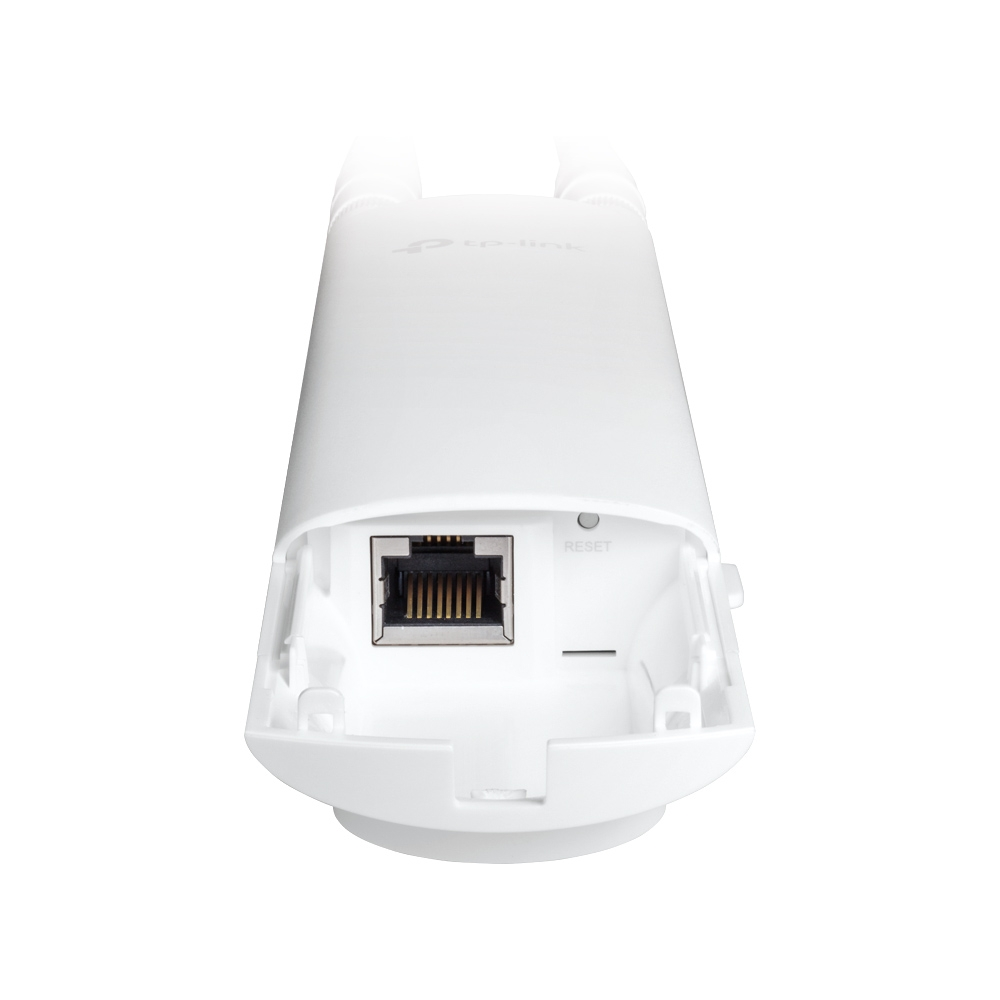
\includegraphics[width=0.45\textwidth]{images/components/EAP225/EAP225-Outdoor-Port.jpg}
    \caption{EAP225-Outdoor bottom port panel, showing the Ethernet port and RESET button.}
    \label{fig:eap225-port}
\end{figure}

\begin{figure}[H]
    \centering
    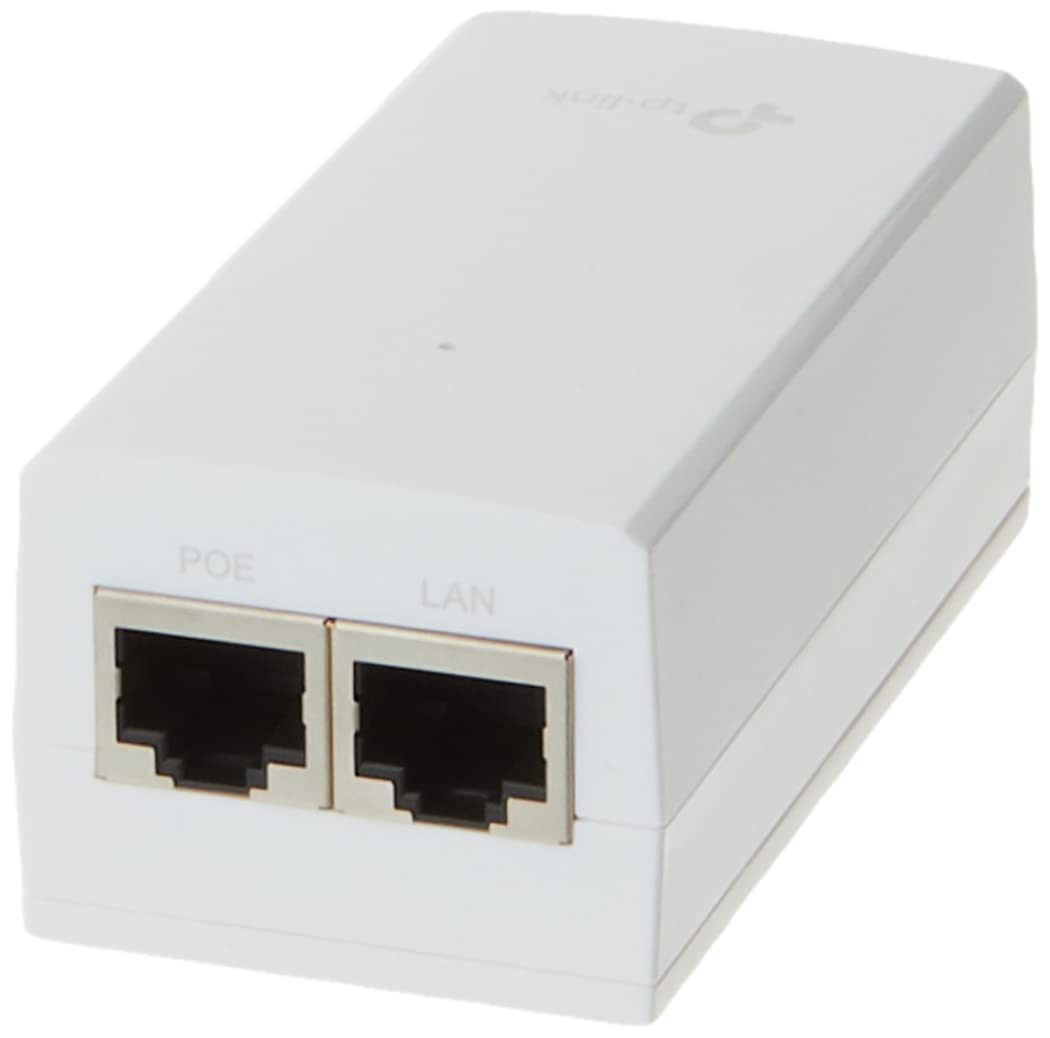
\includegraphics[width=0.45\textwidth]{images/components/EAP225/EAP225-Adapter.jpg}
    \caption{Passive PoE adapter with POE output (to access point) and LAN input (to basestation).}
    \label{fig:eap225-adapter}
\end{figure}

\begin{figure}[H]
    \centering
    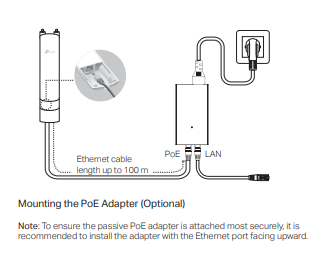
\includegraphics[width=0.8\textwidth]{images/components/EAP225/TP-Link-Diagram.png}
    \caption{EAP225-Outdoor wiring diagram. An Ethernet cable (up to 100\,m) runs from the access point to the POE port on the adapter; the LAN port on the adapter connects to the basestation computer \autocite{EAP225OUTDOOR}.}
    \label{fig:eap225-diagram}
\end{figure}

\subsubsection{Physical Connection}

\begin{enumerate}
    \item Run an Ethernet cable from the port on the bottom of the EAP225-Outdoor (Figure \ref{fig:eap225-port}) to the \textbf{POE} port on the passive PoE adapter (Figure \ref{fig:eap225-adapter}).
    \item Connect a second Ethernet cable from the \textbf{LAN} port on the adapter to the basestation computer's Ethernet port.
    \item Plug the PoE adapter into a power outlet. The access point will power on via the Ethernet cable.
\end{enumerate}

\notebox{The Ethernet cable between the EAP225-Outdoor and the PoE adapter can be up to 100\,m in length, as shown in Figure \ref{fig:eap225-diagram}.}

\subsubsection{Access Point Configuration}

Once the hardware is connected and the access point is powered:

\begin{enumerate}
    \item On the basestation, open a web browser and navigate to the EAP225-Outdoor's default management IP address (refer to the device label or the TP-Link Omada documentation \autocite{EAP225OUTDOOR} for the default address).
    \item Log in with the default credentials and follow the setup wizard to configure the network name (SSID) and password for the wireless network the ASV will connect to.
    \item Apply the settings and allow the access point to restart if prompted.
\end{enumerate}

\subsubsection{Internet Sharing}

To allow devices connected to the access point's wireless network to reach the internet, the basestation's network connection must be shared over Ethernet:

\begin{enumerate}
    \item On the basestation, open \textbf{Network and Sharing Center} (Windows) or the equivalent network settings panel.
    \item Locate the active internet-facing network adapter (e.g., Wi-Fi).
    \item Open its properties, navigate to the \textbf{Sharing} tab, and enable \textit{Allow other network users to connect through this computer's Internet connection}, selecting the Ethernet adapter connected to the PoE adapter as the home network connection.
\end{enumerate}

\warningbox{Internet sharing exposes the basestation's internet connection to all devices on the access point's network. The team is reviewing whether this configuration should be restricted for security reasons.}

\notebox{The HumberASV team is evaluating automating the access point configuration step using Selenium to reduce manual setup time at competition.}
